\chapter{Power system security}
\label{ch:security}
\adjustmtc
\adjustmtc
\minitoc

This chapter introduces the concept of power system security and reviews how power system security can be assessed.

Power system security is quite a broad topic, therefore section~\ref{sec:Security_and_threats} reminds the definition of security and gives the main issues that can challenge system security. Section~\ref{sec:traditionalSecurity} then describes the deterministic methods currently used by TSOs to assess power system security and discusses their limitations and the need for probabilistic methods.

Probabilistic methods are more powerful than deterministic ones, but this comes at the cost of increased complexity. As discussed in the introduction, probabilistic methods are based on the concept of risk that is defined for a given contingency as the product of the frequency at which the contingency occurs and its potential consequences. However, as the consequences of a contingency typically depend on the initial state of the system (generator setpoints, power flows, assets availability, etc.), they have to be assessed for a variety of possible system states.

Probabilistic methods thus face three challenges that do not exist in deterministic methods. The first is that, since probabilistic methodologies do not require the system to be secured against all considered contingencies, they often consider more contingencies. The selection of contingencies and the estimation of their frequency is discussed in section~\ref{sec:contingencies}. The second challenge is to generate a series of likely system states to apply contingencies to and to estimate the probability density function of those states. This is discussed in section~\ref{sec:init_state}. The third challenge is to quantify the potential consequences of a contingency for a given initial system state. This requires to simulate cascading outages which is notoriously hard and is discussed in section~\ref{sec:cascading}. Also, it might be useful to translate the impact of a cascade on the grid (\eg in terms of MW of load shed) into its impact on society (\eg amount of energy not served (in MWh), total societal cost (in €)). This is discussed in section~\ref{sec:blackout_cost}.

Finally, this chapter concludes with a summary of the main gaps in the literature on probabilistic security assessment which this thesis will try to fill.



\section{Power system security and causes of insecurity}
\label{sec:Security_and_threats}

Power system reliability is based on two concepts: adequacy and security. A power system is said to be adequate if it always has enough generation and transmission capacity to satisfy the electricity demand. And it is said to be secure if it is able to withstand contingencies without consequences for its users. Adequacy and security are seemingly similar concepts which are better differentiated by an example.

Figure~\ref{fig:security_vs_adequacy} shows a very simple power system that consists of one bus with two generators connected via 2 lines to a second bus with one generator and one load. This system is N-1 adequate because it can lose any single element (generator or line) and still have enough generation and transmission capacity to satisfy the 300~MW load. For example, if one of the two line is lost, the other line can still transfer 200~MW from the bus on the left to the bus on the right, which, together with the 100~MW available on the right bus, can fully satisfy the 300~MW load.

\begin{figure}[h]
    \centering
    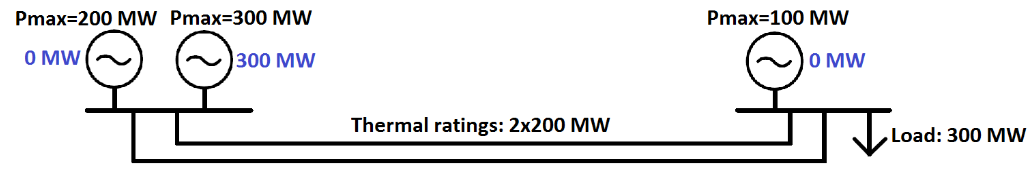
\includegraphics[width=\linewidth]{Figs/Security_vs_adequacy.png}
    \caption{Comparison of security and adequacy~\cite{adequacy_vs_security}. The system is adequate for all N-1 conditions but not operated in an N-1 secure way.}
    \label{fig:security_vs_adequacy}
\end{figure}

Adequacy thus mainly depends on the installed capacities of generators and transmission lines. Security on the other hand, also depends on how the system is operated. In this example, we assume one generator on the left bus is producing the total load of 300~MW and the other generators are turned off (typically because they are more expensive to run). 300~MW are thus transferred from the left bus to the right one. If one of the two lines suddenly fails, those 300~MW will all go through the second line that is only rated for 200~MW. That line will then likely trip (either by being disconnected by some protection system, or by heating, sagging, and entering in contact with vegetation, causing a short-circuit), separating the 300~MW generator and the load leading to a blackout (generators on the left bus no longer connected to the load, and generator on the right bus turned off and too small to satisfy the load).

This highlights an important concept for power system security that is cascading outages. In the above example, the second line is lost, not because of a defect in the line itself, but as a consequence of the loss of the first line. In this case, the loss of a single line causes a complete blackout of the system even though there was still enough generation and transmission capacity to satisfy the load.

Here, the cascading mechanism at play is the trip of lines due to overload. Depending on the severity of the overload, a line might trip after just a few seconds or after a few tens of minutes. An overloaded line can trip either because (i) one of its protection systems operates (\eg line overload protection, distance protection), or (ii) because it overheats, sags and enters in contact with the ground or vegetation causing a short-circuit. In the latter case, power system operators might be able to relieve overloads by redispatching the system: in the example, by ramping up the power production on the right bus such that only 200~MW has to be transferred from the left one. In the former case (trip of the second line after only a few seconds), there is not enough time and only automatic corrective actions defined in advance might be able to save the system.

There are other cascading mechanisms that have overlapping time scales and can thus interact. They are strongly linked with power system stability concepts that are briefly reminded below~\cite{StabilityDefinition, StabilityDefinitionRevised} and summarised in Figure~\ref{fig:stability_classification}.

\begin{figure}
    \centering
    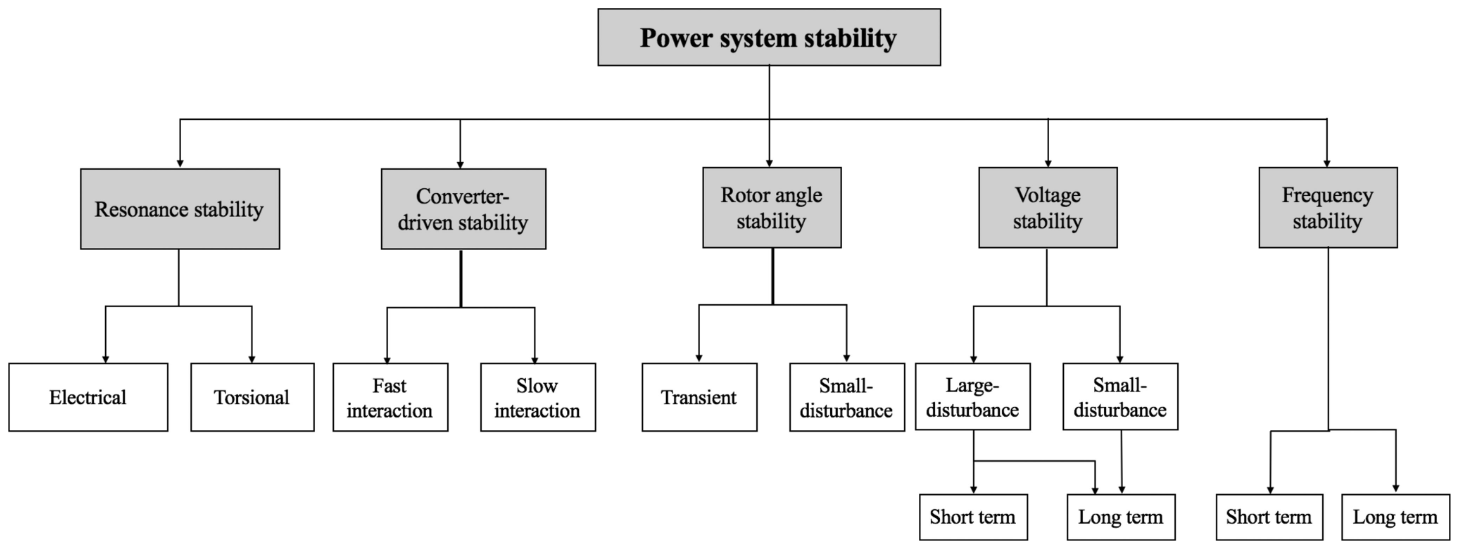
\includegraphics[width=\linewidth]{Figs/StabilityClassification.png}
    \caption{Classification of power system stability~\cite{StabilityDefinitionRevised}}
    \label{fig:stability_classification}
\end{figure}

\begin{itemize}
    \item Frequency stability is the ability of a power system to maintain a steady frequency following imbalances of load and generation. In power systems, the balance between the energy produced by generators and the energy consumed by loads should always be neutral. If there is a lack of energy produced (\eg following the sudden loss of a generating unit), the missing energy will initially be taken from the kinetic energy of synchronous generators that will thus slow down, decreasing system frequency. If generators slow down too much, they will have to disconnect themselves to avoid damage, worsening the system imbalance and thus causing a cascading outage. For large imbalances, the inertia of synchronous generators can only maintain an adequate frequency for a few seconds. Generators thus have to quickly ramp up (or down) to stabilise the frequency. Depending on the generator technology, quick bursts of production might not be sustainable, and in the longer term, the production will have to be complemented by slower ramp up of other generators and/or by turning on other generators.
    \item Voltage stability is, as the name implies, the ability of a system to maintain steady voltages close to their nominal values at all buses of the network. This ability is limited by the voltage drops that occurs when (active and/or reactive) currents flows through inductances of the transmission network. Voltage stability strongly depends on the behaviour of loads and distribution tap changers. Indeed, for a purely resistive load (\eg electric heater), \(P = \frac{V^2}{R}\), thus if voltage decreases by 5\%, the current and power consumed by the load will decrease by 5 and approximatively 10\% respectively, helping voltage stability. If a load has a constant power behaviour (\eg power electronics), the same voltage drop will lead to an increase in current of 5\%, further aggravating the voltage drop and potentially leading to a cascade. Voltage stability is often split in short-term and long-term issues associated with the short-term and long-term behaviour of loads.
    \begin{itemize}
        \item Short-term voltage stability depends mostly on the behaviour of directly-connected induction motors (motors connected through power electronics have a significantly lower impact on voltage stability). When a fault occurs in a power system, low voltages arise in the neighbouring area, induction motors thus slow down as they are no longer able to generate enough electromagnetic torque to match the load torque. When the fault is cleared, motors reaccelerate, but temporarily draw additional current to do so. This can slow down the voltage recovery and even cause a voltage collapse in systems with a high share of induction motors.
        \item Long-term voltage instability occurs when loads try to restore their consumption after a voltage decrease. For example, electric heaters behave as resistive loads in the short term, so reduce their consumption when voltage decrease. However, in the long-term, this causes a decrease in temperature and thermostats thus act to return to the initial power consumption. Other important devices in long-term stability are on-load tap changers that try to recover distribution-level voltages (thus load) when transmission-level voltages are low, and over-excitation limits of generators that limit their reactive power production in the long-term to avoid overheating of the stator and/or of the rotor.
    \end{itemize}
    \item Angle stability is the ability of synchronous generators to remain in synchronism after disturbances. A machine keeps synchronism if the electromagnetic torque is equal and opposite to the mechanical torque delivered by the prime mover. Angle stability can be challenged by both small and large disturbances.
    \begin{itemize}
        \item Large-disturbance angle instability or transient instability occurs when the electromagnetic torque is insufficient which typically happens when the generator is not able to push enough electric power to the grid following loss of transmission elements and during faults.
        \item Small-signal oscillatory instability is generally caused by a lack of damping but can have many causes. Local oscillations occur when a single generator oscillates with the rest of the grid. The damping of these oscillations depend on the control systems of the generator, its power output, and the strength of the grid as seen by the generator. Global issues can be much more complex and occur when multiple generators or groups of generators oscillate against each other.
    \end{itemize}
    \item Converter-driven instability and resonance instability are new categories of instabilities that have been defined following the increasing use of power electronics (HVDC lines, FACTS devices, and inverter-based generation such as solar and wind). Power-electronic-based controls can be much faster than synchronous generator controls and can thus cause oscillations with a frequency of a dozen Hz to hundreds of kHz. As a point of comparison, frequency, voltage and angle stability are affected by phenomena with a timescale from 100ms to a few hours.
\end{itemize}

During severe disturbances, there can be interactions between different types of instabilities. For example, after the loss of a line near a large generator, voltage issues might limit the amount of power that the generator can export leading to a loss of synchronism of this generator (angle instability). The loss of this generator then causes a load generation imbalance that can lead to frequency instability.

% Fig with phenomena time ranges? (\eg from new stability classification paper)

Due to the possible interactions between the different types of instabilities, once a cascade is initiated, it is difficult to predict how it will propagate and when it will stop. In a deterministic security assessment, this does not pose any challenge because it is considered not acceptable for the considered contingencies to lead to large cascading outages. In a probabilistic assessment however, it might be acceptable for a given contingency to lead to a cascading outage, but only if the final consequences are not too big and/or if the frequency of occurrence of the cascading outage is sufficiently small.


\section{Deterministic security assessment}
\label{sec:traditionalSecurity}

In a traditional deterministic security assessment, a power system is deemed secure if it can withstand a set of ``credible contingencies'' without affecting customers nor violating security limits~\cite{N-1-ENTSOE}. This definition relies on three pillars that will be compared with probabilistic methodologies in the next section.

\begin{itemize}
    \item No consequences: A secured contingency should not lead to the disconnection of load nor to the violation of security limits. The definition of security limits differs from TSO to TSO, but typically require to have a steady-state voltages in an acceptable range (\eg the voltages at all buses should be between 0.95 and 1.05pu) and the absence of equipment overload and instabilities. These security limits ensure good power quality for end-users and normally guarantee that no cascading outage will develop (off-nominal voltages, overloads and loss of stability can all cause additional assets to trip, leading to a cascading outage).

    Depending on the TSO, the security limits should be satisfied without the need for corrective actions (preventive approach) or after corrective actions have been implemented (corrective approach). In case (non-automated) corrective actions are used, it makes sense to define different security limits before and after the corrective actions are implemented (\eg voltages between 0.9 and 1.1~pu just after the disturbance, and between 0.95 and 1.05 after corrective actions) to make sure that the system does not cascade before corrective actions have time to be implemented.

    \item A list of credible contingencies: The set of credible contingencies is often based on the famous N-1 criterion, \ie the power system should be able to withstand the loss of any single element (out of N), but elements can be added or removed from this list. ENTSO-E~\cite{ACER_CSAM} classifies contingencies into
    \begin{itemize}
        \item Ordinary contingencies: these include the loss of a single line, transformer, generating unit, or HVDC system. The system should normally always be able to withstand these contingencies (base N-1 criterion)\footnote{In the Nordic countries, remote areas might be operated in N-0 only as it would be too expensive to duplicate some very long lines to guarantee the security of supply of small loads. In other countries (\eg Belgium), violations of the N-1 security rule might also be accepted during maintenances, provided that N-1 contingencies only lead to load shedding in a small part of the grid and that power can be restored by interrupting the maintenance and putting back the asset in service.}.
        \item Exceptional contingencies: loss of multiple elements due to a common-mode failure. These events can be further categorised into events with a permanent occurrence increasing factor, and events with a temporary risk increasing factor. Temporary risk increasing factors are generally linked to specific operating conditions or weather conditions. For example, during wind storms, tower failures are more likely, so the loss of multiple overhead lines built on the same tower can temporarily be included in the contingency list. On the other hand, permanent risk increasing factors are related to specific geographical locations and design conditions. For example, in Belgium, faults on 400kV busbars are considered as exceptional contingencies with a permanent risk increasing factor because, while rare, they can have significant consequences on grid security.
        \item Out-of-range contingencies: loss of multiple elements without a common-mode failure, \eg loss of two independent lines, transformers, etc. These contingencies are typically not considered because it is considered uneconomical to guarantee that they have no consequences as they rarely occur in practice.
    \end{itemize}
    \item A list of pre-contingency states: To simplify the analysis, security assessment is typically performed on a small set of representative or ``umbrella states''. The set of those states should be defined according to the following criteria~\cite{CIGREreviewOfTools}.
    \begin{itemize}
        \item Credibility: the pre-contingency states should be reasonably likely to occur.
        \item Severity: the pre-contingency states considered should lead to the worst-case performance of the system for the considered contingencies.
        \item Representativity: the pre-contingency states and contingencies considered should cover the main weaknesses of the system and phenomena observed during past outages.
    \end{itemize}
    Thirty years ago, it might have been sufficient for some TSOs to only consider one or two pre-contingency states because there was only one main source of variability in the grid: the load. A list of pre-contingency states simply based on expected peak and minimum load for a given time horizon could thus satisfy the criteria of credibility, severity, and representativity. Nowadays, there are however more sources of variability and uncertainty. Most importantly, (i) the growing installed capacity of renewable but intermittent energy sources whose production is difficult to perfectly forecast, and (ii) market liberalisation and increased cross-border electricity trades that make it more difficult to predict what generators will be dispatched at a given moment.

    Due to this high variability, it is becoming more difficult to choose a set of pre-contingency states and contingencies that simultaneously satisfy all the above criteria. Indeed, the variability of renewable energy sources greatly increases the number of possible pre-contingency system states. Consequently, the number of possible system issues also increases. If the considered set is too small or does not consider a sufficiently high variety of system configurations, important issues might be missed. On the other hand, some issues might only appear during very rare system configurations (and assuming a contingency occurs when the system is operating in such state). So, designing the system around a set of extreme cases might be uneconomical.
\end{itemize}


\section{Probabilistic security assessment}
\label{sec:probabilisticSecurity}

As opposed to deterministic methods, in a probabilistic security assessment, one does not need to make an a priori decision on what ``credible'' contingencies should be secured nor on which system states security should be assessed. Instead, probabilistic methods consider larger sets of contingencies and system states, estimate the risks associated with each scenario (combination of a contingency and initial state), and thus provide a better basis to be used to provide recommendations on how to best reduce these risks. As such, they rely less on the complex \emph{art} of defining credible scenarios, but more on the complex \emph{science} of estimating the frequency and consequences of scenarios. Also, by quantifying the risk (in terms of average energy not served to consumers (in MWh/y) or societal costs (in M€/y)), they allow for easier decision-making: what is the cost of risk mitigation measures vs. how much the risk will be decreased if those actions are implemented.

The necessity to transition from deterministic security assessment methodologies to probabilistic methodologies has been acknowledged in the industry and the literature. For example, the ACER decision 07/2019 of 19 June 2019 requires the European transmission system operators to develop a probabilistic approach for risk assessment of power systems by 2027~\cite{ACER}. In the literature, research on probabilistic security assessment has been active for more than two decades and is reviewed in this section.

Probabilistic methodologies in the literature differ in part by ``how probabilistic'' they are. Indeed, ``fully probabilistic'' methodologies and the historical implementation of the N-1 criterion differ in multiple aspects that are summarised below, with many methodologies having been developed between the two extremes.

\begin{itemize}
    \item Contingencies: as discussed above, in a deterministic security assessment, the system is said to be secure if it can withstand any contingency from a list of credible contingencies. This is the same as if all contingencies in the considered list were assumed to have the same frequency of occurrence, and as if the contingencies not in the list were assumed to have a null frequency of occurrence. On the other hand, in a probabilistic approach, the frequency of occurrence of contingencies is estimated and used to estimate the risk they pose to the grid. It should however be noted, that even in deterministic methods, there is already a form of qualitative risk assessment in the selection of considered contingencies (\eg exceptional contingencies with temporary and permanent risk factors).
    \item Operating conditions: deterministic studies consider a contingency to be secure if it is secure for a given list of ``umbrella states'', while probabilistic methodologies consider the probability of occurrence of the grid being in a given state to estimate the associated risk. Again, even with deterministic methods, there is some form of qualitative risk assessment in the selection of considered states, especially now that TSOs consider more states to account for ``low'' and ``high'' winds, solar, etc.
    \item Consequences: there are four main ways consequences can be estimated.
    \begin{itemize}
        \item No cascading allowed: any scenario that leads to cascading (\eg overloaded line) is considered unacceptable.
        \item Small cascades allowed: some cascading can be allowed but only if it leads to no or little load shedding. This is the approach currently used by most TSOs.
        \item Large cascades, single-path methods: large cascades can be allowed even with significant consequences if the associated risk if small. The cascades are simulated in a ``deterministic'' manner, also referred to as the single-path approach. This assumes that one can accurately simulate how a given cascade will propagate and what will be its consequences.
        \item Large cascades, multi-path methods: multi-path methods acknowledge the fact that many modelling uncertainties can significantly affect the propagation of cascades and their final consequences and thus simulate them in a ``probabilistic manner''. For example, if, at a given point of the cascade, two lines are overloaded, the single-path approach could assume that the most overloaded line will trip first or that both lines will trip simultaneously. In practice, tripping of overloaded lines can be caused by lines heating, sagging, and entering in contact with the ground or vegetation. Whether overloaded lines trip and in which order thus depend on the severity of the overload, but also on more uncertain factors such as weather (\eg wind cooling down lines) and vegetation height. Multi-path methods handle this uncertainty by simulating multiple possible cascade evolutions, \eg one where the first overloaded line trips first, and one where the second line trips first, each associated with a given probability.
    \end{itemize}
\end{itemize}

As discussed above, probabilistic methods typically consider higher order contingencies than deterministic methods. It is thus necessary to model them and their root causes to estimate their frequency of occurrence, this is discussed in section~\ref{sec:contingencies}. Also, they consider more system states, so it is also necessary to generate these system states and to estimate their probability density function (section~\ref{sec:init_state}). Finally, for all considered scenarios (contingency and state), the potential consequences of a contingency on a given state have to be quantified. This requires to predict if a cascading outage will occur, if it does to predict how far it will propagate and what will be the final consequences for the users (in terms of energy not served or monetary cost for society). The simulation of cascading outages is thus discussed in section~\ref{sec:cascading}.

\subsection{Contingency selection}
\label{sec:contingencies}

There are many contingencies that can affect power systems, often classified using the N-x formulation, \ie by counting the number x of elements (out of N initially available) that are lost following a contingency. Different classes of contingencies have different root causes and therefore different frequencies of occurrence~\cite{ContingencyTypes}. This section lists the main types of contingencies\footnote{Note that, as for many security-related concepts, the classification is not standardised.}, explains how to estimate their frequency, and discusses the main challenges that they pose when integrating them in a probabilistic security assessment. This is also summarised in Table~\ref{tab:contingencies}.


\paragraph*{N-1 contingencies} are the simplest and the most common contingencies that can occur in power systems. They are caused by single failures of transmission or generation assets. A typical example of N-1 contingency is the loss of a line following a lightning strike on the line. N-1 contingencies are relatively frequent (not for individual assets, but on the scale of a country), so TSOs often have statistics that allow for the estimation of their frequency of occurrence. For example, in France, it is estimated that line faults occur with a frequency of 2.5 occurrences\footnote{This figure includes all types of line faults (single-phase-to-ground, three-phase, etc.). In this thesis, all line faults are modelled as three-phase faults, although the majority of line faults are single-phase-to-ground. This is a quite conservative assumption as three-phase faults are more challenging from a system stability perspective (it can however be noted that protection systems might be more likely to misoperate for single-phase faults compared to three-phase ones~\cite{Alexandre_PMAPS}). Also, auto-reclosing of lines is not considered. Given these conservative assumptions, it might thus make sense to use a smaller value for the frequency of N-1 contingencies. For N-k contingencies (described below), for example a line fault followed by a breaker failure to open, such hypothesis make more sense as auto-reclosing will not be attempted and the three phases will need to be disconnected.} per year and per 100~km of line~\cite{FaultStatisticsFrance}. In a probabilistic security assessment, it can be noted that the frequency of occurrence of contingencies can be indirectly correlated to the system state. For example, in Finland, lightning strikes happen mostly during the summer~\cite{GridPSA}, so system states that occur more often in the summer are more at risk. Another challenge posed by N-1 contingencies in probabilistic assessment is that, since they are relatively frequent, it must be checked that they pose little consequences in a very large majority of system states to make sure that the risk (product of frequency and consequences) they cause is acceptable.

% Often single phase faults, but consider three-phase because easier to simulate and conservative.

% \begin{table}
%     \centering
%     \caption{Summary of the categories of contingencies and the main challenges in integrating them in a probabilistic security assessment}
%     \label{tab:contingencies}
%     \begin{tabularx}{\linewidth}{@{}sslllB@{}}
%     \toprule
%     \begin{tabular}[c]{@{}l@{}}Contingency\\ type\end{tabular} &
%         Main causes &
%         \begin{tabular}[c]{@{}l@{}}Average frequency \\ of individual\\ contingencies (/y)\end{tabular} &
%         \begin{tabular}[c]{@{}l@{}}Number of\\ contingencies\end{tabular} &
%         \begin{tabular}[c]{@{}l@{}}Total\\ frequency\\ (/y)\end{tabular} &
%         Challenges \\ \midrule
%     N-1                 & Single failures      & 1    & 1000 & 1000     & High frequency \\[0.5cm]
%     N-1-1               & Independent failures & 0.00003     & 1,000,000 & 30 & Number of contingencies \\[0.5cm]
%     N-k (k = 2-5)       & Common-mode and hidden failures & 0.01 & 10,000 & 100   & Modelling of causes \\[0.5cm]
%     N-1 (delayed clearing) & Hidden failures & 0.1 & 1000 & 100   & Intermediate between N-1 and N-k \\[0.5cm]
%     N-K (K \(\gg\) 2)   & Hurricanes, earthquakes, cyber-attacks & Variable  & Variable & Variable & Modelling of causes and restoration \\[0.5cm]
%     Other contingencies & Black clouds              & N/A    & N/A & N/A & Modelling of causes \\ \bottomrule
%     \end{tabularx}
%     \end{table}

\afterpage{%
\clearpage% Flush earlier floats (otherwise order might not be correct)
% \thispagestyle{empty}% empty page style (?)
\begin{landscape}% Landscape page
\centering
\begin{table}
\caption{Summary of the categories of contingencies, order of magnitude of their frequency and number (for a system with 1000 branches), and main challenges in integrating them in a probabilistic security assessment}
\label{tab:contingencies}
\begin{tabularx}{\linewidth}{@{}lslllB@{}}
\toprule
\begin{tabular}[c]{@{}l@{}}Contingency\\ type\end{tabular} &
    Main causes &
    \begin{tabular}[c]{@{}l@{}}Average frequency \\ of individual\\ contingencies (/y)\end{tabular} &
    \begin{tabular}[c]{@{}l@{}}Number of\\ contingencies\end{tabular} &
    \begin{tabular}[c]{@{}l@{}}Total\\ frequency\\ (/y)\end{tabular} &
    Challenges \\ \midrule
N-1                 & Single failures      & 1    & 1000 & 1000     & Security must be guaranteed for a large set of system states \\[0.5cm]
N-1-1               & Independent failures & 0.00003     & 1,000,000 & 30 & Very high number of possible contingencies, but most do not pose security risks \\[0.5cm]
N-k (k = 2-5)       & Common-mode and hidden failures & 0.01 & 5000 & 50   & Modelling of common-mode and hidden failures \\[0.5cm]
N-1 (delayed clearing) & Hidden failures & 0.1 & 1000 & 100   & Intermediate between N-1 and N-k \\[0.5cm]
N-K (K \(\gg\) 2)   & Hurricanes, earthquakes, cyber-attacks & Variable  & Variable & Variable & Modelling of the causes of contingencies and of the recovery of the system after contingencies \\[0.5cm]
% Other disturbances & Black clouds              & N/A    & N/A & N/A & Modelling of the causes of contingencies \\
Complex contingencies & Various              & N/A    & N/A & N/A & Modelling of the causes of contingencies \\ \bottomrule
\end{tabularx}
\end{table}
\end{landscape}
\clearpage% Flush page
}

\paragraph*{N-1-1 contingencies} are a combination of two N-1 contingencies that occur in relatively quick succession. Power systems are typically designed to be N-1 secure. However, once an N-1 contingency occurs, the system can degrade to an N-0 secure state. When this happens, operators will try to perform corrective actions to bring back the system to an N-1 state. But if a second contingency happens before operators have time to act, it might challenge system security. If contingencies are assumed to be independent, the frequency of an N-1-1 contingency that consist in contingency \(i\) occurring after contingency \(j\) but after a time less than \(T\) is

\begin{equation}
\label{eq:N-1-1_frequency}
    f_{i,j} = \lambda_i  (1-e^{-\lambda_j T})
\end{equation}
\noindent where \(\lambda_i\) is the (\eg yearly) frequency of occurrence of contingency \(i\), and \((1-e^{-\lambda_j T})\) is the probability that contingency \(j\) occurred in the last \(T\) minutes. In static security assessments (\ie assessments that consider asset ratings (and steady-state voltage limits), but not dynamic stability issues), such contingencies can be considered as N-2 contingencies as they have the same effect. This is not the case in dynamic security assessments, because the time delay between the occurrence of the two contingencies usually makes the N-1-1 contingency less severe than if the two contingencies occurred at the same time. N-1-1 contingencies that occur with significant time delay between the two contingencies (\ie leaving enough time to perform corrective actions) can also be considered to check that it is indeed possible to bring back the system to an N-1 secure state after a first contingency. (This is mostly done in static security assessments, for example in the US~\cite{ContingencyTypes}.)

Individual N-1-1 contingencies have an extremely low frequency of occurrence but many possible N-1 contingency combinations are possible leading to a very high number of possible N-1-1 contingencies. Indeed, from (\ref{eq:N-1-1_frequency}), if two contingencies have a frequency of 1 per year, and if we assume that it takes on average 15 minutes for operators to bring back the system to an N-1 secure state (\(T = 15 \text{ minutes}\)), then these two contingencies will lead to N-1-1 conditions every 30 per \emph{million} years. But, if there are \(\text{N} = 1000\) possible N-1 contingencies, there are \(N(N-1) \approx 1,000,000\) possible N-1-1 contingencies. So, in total, N-1-1 contingencies would happen 30 times per year in this example. This is the same order of magnitude as the total frequency of N-k events (see Table~\ref{tab:contingencies} and next paragraph)\footnote{In~\cite{ContingencyMotifs}, authors analysed 19 years of historical outage data recorded in the Bonneville Power Administration power system and observed that when two lines failed in a one-hour interval, in 81\% of the cases, the two lines were adjacent, indicating an N-k contingency (or small cascade).}, however, on average, N-1-1 contingencies have less chance to have consequences than N-k contingencies. Indeed, especially in large systems, two N-1 contingencies occurring at opposite ends of the system will unlikely lead to consequences. The risk of independent N-1-1 contingencies can thus often be neglected compared to N-k contingencies. But if they are considered anyway, screening techniques should be used to limit the number of combinations to simulate~\cite{VittalN-1-1}.

N-1-1 contingencies can become much more likely when they are no longer independent. For example, in 2021, two parallel interconnections between France and Spain where lost at two minutes of interval due to a wildfire. This initiated a cascade that led to the separation of the two systems~\cite{ENTSOEIbericSplit2021}. The system should have preventively been made N-1-1 secure in the vicinity of the fire to avoid this incident, but system operators were unaware of the fire due to lack of communication from the fire department.


\paragraph*{N-k contingencies (k = 2-5)} consist in the simultaneous loss of k elements. N-k contingencies virtually cannot occur due to independent contingencies (limit of \(T \to 0\) in (\ref{eq:N-1-1_frequency}) gives a null frequency), and instead occur due to common mode and hidden failures. A common mode failure is the simultaneous failure of several elements due to a single root cause. For example, two lines sitting on the same tower will be lost if the tower is lost. Also, busbar faults are often considered to be N-k contingencies because all lines connected to the busbar might need to be disconnected to clear the fault. As seen from those examples, N-k contingencies often imply the loss of elements located in close proximity (parallel lines, adjacent lines) and are thus often more severe than N-1-1 contingencies.

A hidden failure is a failure that does not directly impact system operations but increases the chance of failure of equipment to perform an on-demand function. Hidden failures are of particular concern in protection systems. Indeed, protection systems need only to operate when a fault occurs in a given element of the grid. If a protection system fails, a backup protection system will need to operate to clear the fault and avoid equipment damage. Backup protections are however slower than primary protections and often trip multiple non-faulted elements. Protection systems and their failure modes will be discussed in much more detail in chapter~\ref{ch:protections}.

% Mention Ian Dobson paper \url{https://ieeexplore.ieee.org/stamp/stamp.jsp?arnumber=10054456}, \url{https://arxiv.org/pdf/2209.02192} but (identified) critical lines might have more reliable protections (\eg double differential (independent sets of relays), or even SIPS) than less critical ones (\eg single distance protection with overcurrent backup). (Time resolution of data (1min) makes it difficult to differentiate between independent events and cascade. Actually, probably need some manual postprocessing to separate the two)

The importance of hidden failures is highlighted by the study of historical blackouts. For example, Ref.~\cite{CascadingMethodoAndChallenges} observed that out of the 26 major unreliability events reviewed in a CIGRE (Conseil international des grands réseaux électriques) report\footnote{Most of these disturbances affected more than one million customers and led to at least 5~GW of power not served.}~\cite{majorBlackouts}, 19 of them were triggered by losses of single transmission elements albeit many of these events were exacerbated by other problems. Further analysis shows that 18 of the 26 events were caused or aggravated by hidden failures. The same observation can be made for smaller scale events. For example, the study of significant disturbances reported by the NERC~\cite{NERCDisturbancesReport} (North American Electric Reliability Corporation) in the period from 1984 to 1988 and summarised in~\cite{ZoneVulnerability} indicates that protective relay misoperations were involved, in one way or another, in 73.5\% of disturbances\footnote{This includes both spontaneous operation of protections (without preceding event) and hidden failures. However, as power systems are designed to be N-1 secure, spontaneous operations should usually not have consequences.}.


\paragraph*{N-1 contingencies with delayed fault clearing} are similar to N-k contingencies in that they are caused by a single fault that is not cleared by the primary protection system of the faulted element. The difference is that the backup is able to clear the fault by disconnecting only the faulted element (but still requires more time than the primary protection to do so). They are often more likely than N-k contingencies (less severe failure of protection system) but have a smaller impact on the system\footnote{No publicly available statistics were found regarding the rate of N-1 contingencies with delayed fault clearing. The frequency of 0.1/y in Table~\ref{tab:contingencies} is thus taken as an intermediary value between the one of normal N-1 contingencies and the one of N-k contingencies}. Their relative contribution to the total risk thus depends on the considered power system.


\paragraph*{N-K contingencies (K \(\gg\) 2)} are caused by extreme events such as hurricanes, earthquakes (weather events) and cyber-attacks (man-made events). Such extreme events have a low frequency but can lead to the loss of many assets in a short period of time. The ability of power systems to withstand such events falls out of scope of the topic of security (thus of this thesis), but is included in the topic of resilience. Apart from the larger severity of such events, another difference with security-related events is that it is more difficult for the system to recover from them. Indeed, security-related events can lead to cascading outages and even complete blackouts, but rarely cause damage in transmission equipment and generators. Black start and complete restoration is usually performed in less than 24~hours. While for extreme events, parts of the network might stay deenergised for days or weeks before the necessary repairs can be completed.


% \paragraph*{Other disturbances} are disturbances that do not fall in the above categories. One example of such disturbance is the occurrence of black clouds. (Moving) black clouds can cause large and relatively fast changes in power flows by obscuring photovoltaic panels and causing increased load (lighting, heating), especially when above large cities. Such disturbances weaken the system and can lead to large consequences, especially when combined with the above contingencies. They are not very well documented and thus not considered further in this thesis.


\paragraph*{Complex contingencies} are disturbances that do not fall easily in the above categories. Many historical large disturbances were initiated by such complex contingencies. For example, in 2019, a fault occurred on a 400kV line in the UK and was normally cleared in 80ms. But then, a wind farm located roughly 200 km away from the fault rapidly decreased its production from 799 to 62~MW. Shortly after, a combined cycle gas turbine (located close to the initial fault) was disconnected. This led to a large generation load imbalance that, along with other aggravating factors, led to a frequency decrease and to the disconnection of one million customers~\cite{2019UKBlackout}. This event could be considered as an N-1 contingency as the initial event was a single line fault, but it had the consequences of an N-3 event. It is extremely difficult to predict such events and to estimate their frequency as their root causes can be quite complex (6 months after the occurrence of the UK blackout, the causes of the gas turbine trip were still unknown~\cite{2019UKBlackout}). It is even more difficult to predict these kinds of events since they are expected to be ``only once'' events thanks to the lessons learned from their occurrence. In the UK case, following the blackout and a growing number of cases where generators failed to ride through normally cleared transmission faults (which is a requirement for any transmission-connected generator), the UK grid codes were updated such that generators that failed to meet fault-ride through requirements have to limit their production (possibly to 0~MW, to limit the threat they pose to system security) until they are able to demonstrate that they meet the grid codes~\cite{FaultRideThroughEnforcement}.

% Another example... 2021 split busbar. Sequence, lessons learned

A question that is left open in this thesis is whether we should try to predict such complex events and include them in probabilistic security assessments, or whether security assessments should focus on the more ``classical'' N-1 and N-k contingencies, leaving the more complex contingencies to the defence plans.


\subsection{Generating likely system states}
\label{sec:init_state}

To evaluate the risk associated with a given contingency, it is necessary to predict in what initial state the system could be upon occurrence of the contingency and what are the probabilities of all possible initial states. Mathematically speaking, this requires to have (an approximation of) the probability density function of the system state\footnote{Actually, it would be best to have a probability density function conditioned by the occurrence of the contingency to account for correlations between the occurrence of a contingency and the system state (\eg in Belgium, lightning strikes are more likely to occur during the summer)} (generator outputs, load flows, asset availability, etc.).

Estimating this probability density function is very challenging because it is a high-dimensional function (must account for (active and reactive) power injection at all buses, asset availability, substation topologies) with strong correlations between its variables (especially spatio-temporal correlations between the renewable energy availability at different points in the network). Despite the importance of this step in the probabilistic security assessment work, it has not been studied in details in this thesis. Instead, two of the most potent and popular methods from the literature are described below. The former will be used in the test cases in section~\ref{ch:DPSA}.

The first method has initially been developed in the GARPUR project~\cite{StrathElia, StrathGARPUR} and is now routinely used by some European TSOs and ENTSO-E to perform adequacy studies~\cite{ACER_MC_year, EliaAdequacy}. The methodology consists in, first, using weather data to generate so-called ``Monte Carlo (MC) years''. An MC year is time series realisation of renewable generation availability and load for one year with a typical resolution of one hour. Please refer to~\cite{StrathGARPUR} for more information on how to generate MC years while considering temporal and geographical correlations between renewable outputs and loads. Secondly, for each MC year, a market model is used to determine the commitment of thermal generators. Finally, each year is divided into (\eg hourly) snapshots, and a (security-constrained) optimal power flow is performed on each snapshot to model potential preventive actions taken by operators. All snapshots are saved in a database to be used in the rest of the probabilistic security (or adequacy) assessment. % (\cite{DCAT_2023} also uses weather, but few details given)

The second method consists in fitting an analytical probability density function based on historical data, often using copula to handle correlations. This approach has been extensively studied during the iTesla project~\cite{KonstantelosCopulas, EurostagHPC}. In this project, the complete system state, including substation topologies (and accounting for potential preventive actions performed by operators), was directly inferred from historical data. This can be more accurate than the GARPUR approach, because optimal power flows do not handle well substation topologies (requires many binary variables in the optimisation problem) and operator actions (do not always perform the predicted optimal actions). However, the reliance on historical data makes it a less flexible approach. In particular, it does not allow to model the impact of climate change on the likelihood of droughts and other severe weather events. So it is less adequate for long-term (\eg 10 year horizon) studies. Also, if operating rules are modified (\eg to enhance security as we will discuss in chapter~\ref{ch:DPSA}), historical data on operator actions might no longer be relevant.

% One industry-grade tool worth mentioning is ASSESS~\cite{AssessRTE, AssessNationalGrid} developed by RTE and National Grid (\ie the French and British TSOs respectively). It does not compute the consequences of contingencies (\ie only classify them as acceptable or not), but it generally considers more uncertainties in the pre-contingencies states, and it has a toolbox of statistic and data mining tools that can be used to analyse the results. It is particularly useful to define operational limits by ``drawing a line'' between the acceptable and unacceptable pre-contingencies states. % Little information given (except many probability laws are available --> No correlations?)


\subsection{Simulation of cascading outages}
\label{sec:cascading}

For each combination of initial system state and contingency (called a scenario hereafter) considered in the analysis, it is necessary to quantify what would be the impact of the contingency if it occurred when the system was in the considered initial state. For the scenarios that lead to cascading outages, it can be challenging for two main reasons. The first is that simulating cascading outages requires to simulate the system in very degraded states. This is not needed in deterministic security assessments and thus rarely done by TSOs. Models are thus poorly validated in those degraded states. Moreover, power systems rarely face very degraded states, so there might be a lack of data to validate the models.

The second challenge is that, in some cases, cascading outages might be very sensitive to modelling assumptions. This is because in a cascading outage, many elements are subject to abnormal conditions and thus likely to trip or misoperate. A good example of this is the tripping of lines caused by overload. When a line is overloaded, its temperature increases due to the Joule effect. It thus sags and can then enter in contact with vegetation causing a short-circuit followed by a trip of the line. The line trip causes a redistribution of the power flows and can cause overloads in other lines which contribute to the propagation of the cascade. The redistribution could also resolve some overloads, stopping the cascade propagation. At some point in the cascade, it is likely that multiple lines will be overloaded. In the first probabilistic security assessment methodologies developed, a common assumption was that, in case of multiple overloaded lines, the most overloaded line would trip first. In practice however, slightly less overloaded lines could trip first due to different vegetation height, weather, etc. The trip of a different line can cause a very different redistribution of power flows that causes different lines to be overloaded in the next step of the cascade. The resulting cascade can thus be very different (in terms of size, geographical distribution, impacted elements, etc.) than the one where the most overloaded line was tripped first. This difference is further amplified when we consider the competition between different cascading mechanisms.

In the literature, two main types of methods have been developed to simulate cascading outages: the ones based on a static grid model (section~\ref{sec:QSSmethods}), and the ones based on a dynamic grid model (section~\ref{sec:DynMethods}). These methods are quite different as they have to cope with different limitations. The former have to introduce additional heuristics to approximate dynamic effects while the latter are limited by computation time. Additionally, some methods do not fall in the above categories and are reviewed in section~\ref{sec:OtherMethods}.


% Actually, a lot of different methodologies can be placed under the umbrella of probabilistic methodologies, but the number of uncertainties taken into account can vary greatly. The most straightforward probabilistic assessment method is the contingency enumeration method. It is similar to the deterministic method in that one will assess the security of a list of contingencies (usually larger than in a deterministic assessment, \eg including N-2 events and loss of towers). The difference is that contingencies are associated with a probability. Also, instead of simply classifying contingencies as acceptable or unacceptable, the consequences are usually computed, but in a deterministic manner. Due to the relative simplicity of the methodology and similarity with the deterministic method, it is implemented in most commercial software tools\footnote{At the time of the writing of the CIGRE review~\cite{CIGREreviewOfTools} (2010), all tools used the quasi-steady-state (QSS) approximation (that will be described in section~\ref{sec:QSSmethods}) to evaluate the consequences. Now, some tools (\eg PSS/E~\cite{PSSE} and DIgSILENT PowerFactory~\cite{PowerFactory}) also allow to use dynamic simulations. Due to the simplicity of the method, it is possible to implement it with any tool that has basic scripting functionality.}~\cite{CIGREreviewOfTools}.

% Industry-grade tools only consider the uncertainties related to the initial state and initial contingencies. After the occurrence of a given contingency, the system is simulated in a fully deterministic manner. Those tools are thus unable to consider hidden failures as those manifest after the initial contingency\footnote{The hidden failures that occur just after the initiating event (\eg failure to open a faulted line) could be modelled as part of the initiating events as done in~\cite{Haarla, GridPSA}. This is discussed in section~\ref{sec:DynMethods}. This is however not possible for failures that occur later in the cascade. For those, it is necessary to have a probabilistic simulation of the evolution of the cascade.}.




\subsubsection{Methods with a static grid model}
\label{sec:QSSmethods}

Methods based on a static grid model typically follow a common scheme illustrated in Figure~\ref{fig:QSS_flowchart}. First, the system is initialised at the pre-contingency state, and the initiating contingencies are triggered. Then, the post-contingency state is computed using an (AC or DC) power flow algorithm. If some elements are subject to unacceptable conditions (\eg overload, undervoltage, etc.), those elements are tripped or other remedial actions are implemented (\eg under-voltage load shedding (UVLS), redispatch, etc.). After those disconnections/actions, the state of the system is recomputed. The process is repeated until no more elements are subject to unacceptable conditions or if a full blackout occurs.

\begin{figure}
    \centering
    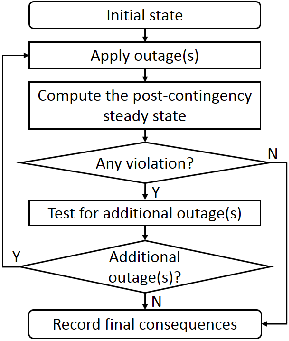
\includegraphics[width=0.4\linewidth]{Figs/QSS_flowchart.pdf}
    \caption{Typical flowchart of static cascading outage methodologies~\cite{Benchmarking2018}}
    \label{fig:QSS_flowchart}
\end{figure}

As the computation cost of a power flow is relatively low (of the order of 1s for large systems), the cost of static methods is also low. This is particularly useful as probabilistic security assessment methodologies require to simulate many scenarios. An obvious limitation is that static methodologies do not directly account for stability issues as they do not perform time-domain simulations. Historically, this was justified by the fact that cascading outages used to often develop in two phases: a slow phase driven by thermal phenomena (line overloads) followed by a fast phase driven by stability issues (frequency, loss of synchronism, etc.). Figure~\ref{fig:BlackoutUS2003} demonstrates this for the case of the 2003 US blackout~\cite{USBlackout2003}. The cascade was initiated at 15:05 by the loss of multiple parallel lines due to heavy loading. One hour later (at 16:05, start time of Figure~\ref{fig:BlackoutUS2003}), two dozen lines were disconnected. Around 16:09 the cascade transitioned to a fast phase and hundreds of elements were disconnected in two minutes. In the light of this blackout, static methodologies are often seen as adequate to model the early stage of cascades, but not their fast phase (where most of the elements and loads are disconnected)~\cite{BenchmarkingStaticVsDynamic}. This has led to the development of hybrid methodologies where the start of cascades is represented with a static model, and the end with time-domain simulations~\cite{TwoLevelPSA, DCATphase1}.

\begin{figure}
    \centering
    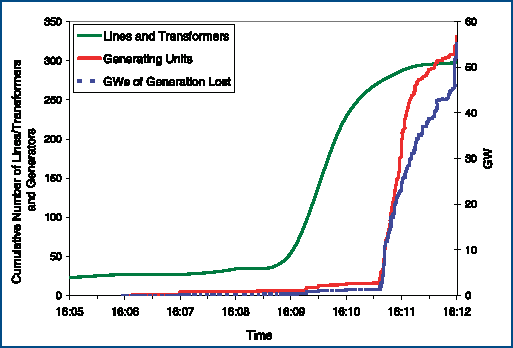
\includegraphics[width=0.7\linewidth]{Figs/USBlackout2003.pdf}
    \caption{Rate of line and generator trips during the cascade that led to the 2003 US blackout~\cite{StabilityDefinitionRevised}}
    \label{fig:BlackoutUS2003}
\end{figure}

A major challenge in the simulation of cascading outages is the handling of ``race conditions''. For example, if at a given step of the cascade, two lines are overloaded, which of the two lines will trip first? Actually, will they trip at all, or will an operator be able to relieve the overloads before lines are tripped? Such race conditions can also occur between different types of cascading mechanisms (\eg will the overloaded line trip before the over-excitation limiter of a generator acts).

% This depends on whether the lines were already overloaded in the previous cascading steps and on variables (weather, vegetation height) that are difficult to model. This race conditions can also occur between different types of cascading mechanisms (\eg will the overloaded line trip before the over-excitation limiter of a generator acts). The handling of these race conditions is made even harder by the fact that QSS simulations have no concept of time (as load flows assume the system is in steady-state).

Handling of race conditions can be performed with either single-path or multi-paths methods. In the former, only the most likely (estimated) cascading path is simulated. For example, some cascading failure simulators consider that when multiple lines are overloaded, the most overloaded one will trip first. Others trip all overloaded lines in one step~\cite{ManchesterNoebels}. In the multi-path, multiple cascading paths are simulated, each associated with a probability and specific consequences. The probability of an overloaded line to trip is often estimated as a function of the current overload value and/or as a function of the line temperature (computed based on past values of the line currents and on weather)~\cite{Henneaux_level1}.

Another important issue in cascading simulators based on static grid models is the handling of cases where the power flow does not converge (only if AC power flow model is used and/or if discrete controls such as tap changers are included in the power flow model). Non-convergences are often caused by voltage issues and thus resolved by shedding load until the power flow converges or using an optimal power flow to find the minimum amount of load shedding necessary to get convergence. In a dynamic simulation, voltage collapses occur in a ``smoother'' manner as voltages are explicitly considered as time-dependent continuous variables. One can thus observe \eg which loads are subject to undervoltages first and thus which tap changers or under-voltage load shedding relays will actually trigger and in which order\footnote{Numerical stability issues can also occur in dynamic simulations but they tend to be rarer. To avoid those issues, one should be cautious of the models used (\eg Ref.~\cite[p93-98]{SongThesis} proposes to replace constant-power loads with restorative loads with a very short time constant). Protections tend to mitigate numerical issues as they disconnect elements are subject to severe conditions (\eg distance protections disconnecting lines during voltage collapse).}.


% To better illustrate QSS methodologies and the challenges they face in modelling race conditions and stability issues, an example of QSS methodology is described and discussed. The example considered is the AC cascading failure model (AC-CFM)~\cite{ManchesterNoebels} that can be considered as one of the spiritual successors of the famous Manchester model~\cite{OriginalManchesterModel}. This model follows a similar procedure to most QSS models, that is it initialises the system, triggers an initiating contingency, and then checks for violations and performs corrective actions until all violations are solved. The steps that are taken to solve violations at a given step of the cascade are illustrated in Figure~\ref{fig:NoebelsFlowchart} and discussed below.

% \begin{figure}
%     \centering
%     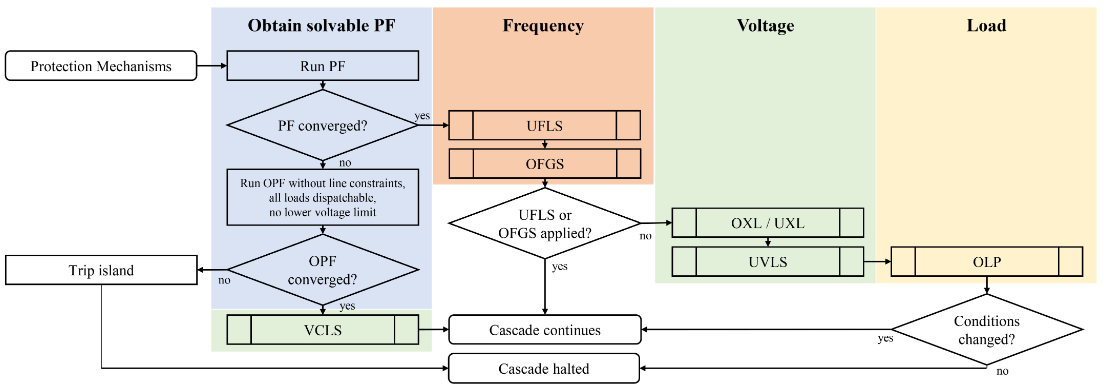
\includegraphics[width=\linewidth]{Figs/NoebelsFlowchart.png}
%     \caption{Flowchart of the AC-CFM methodology~\cite{ManchesterNoebels}. Abbreviations: PF: power flow, VCLS: voltage collapse load shedding, UFLS: under-frequency load shedding, OFGS: over-frequency generator shedding, OXL/UXL: over/under-excitation limiter, UVLS: under-voltage load shedding, OLP: overload protection}
%     \label{fig:NoebelsFlowchart}
% \end{figure}
%
% \begin{itemize}
%     \item Obtain a solvable power flow: AC-CFM uses an AC power flow and AC power flows can fail to converge. This is often caused by lack of reactive power support that causes a voltage collapse. The modelling choice made for the AC-CFM is to use an OPF considering all loads are dispatchable, and to minimise the load shedding necessary to obtain a converging load flow. In a dynamic simulation, voltage collapses occur in a ``smoother'' manner as time is explicitly considered as a continuous variable. One can thus observe \eg which loads are subject to undervoltages first and thus which UVLS relay actually triggers\footnote{Numerical stability issues can also occur in dynamic simulations but they tend to be rarer. To avoid those issues, one should be cautious of the models used (\eg Ref.~\cite[p93-98]{SongThesis} proposes to replace constant-power loads with restorative loads with a very short time constant). Protections tend to mitigate numerical issues as they disconnect elements are subject to severe conditions (\eg distance protections disconnecting lines during voltage collapse).}.
%     \item Frequency: AC-CFM considers that if load-generation imbalances are less than a predefined threshold, the imbalance will be redistributed to the generators (that will increase or decrease their power to restore the imbalance) according to their participation factors. For larger imbalances, load shedding or generation rejection is necessary. In case of lack of generation, the load is reduced uniformly (although prioritisation can be implemented). In case of generation surplus, generating units are disconnected starting with the smallest ones as they tend to more easily lose synchronism. When using dynamic simulations, frequency is modelled explicitly, so it is easier to model the response of generators and to predict when under-frequency load shedding (UFLS) thresholds are reached.
%     \item Voltage: this block has two parts: the over/under-excitation limiters of generators, and UVLS.
%     \begin{itemize}
%         \item OXL/UXL: in AC-CFM, generators that are over/under-excited are made into PQ buses, \ie their reactive power output is considered equal to its limits. In a dynamic simulation, limiters could be modelled similarly. However, as over-excitation limiters protect the generators against excessive heating, a time-delay can be considered. It is also easier to consider the variation of reactive limits with the active power output.
%         \item UVLS: in AC-CFM, load is shed by block until voltages reach acceptable values. If multiple loads are subject to undervoltages, load is shed in all of them simultaneously. In a dynamic simulation, the order of triggering of UVLS relays will depend on the time evolution of voltages at individual load buses. UVLS at one bus can then alleviate or worsen voltage issues in neighbouring buses.
%     \end{itemize}
%     \item Load: in AC-CFM, overloaded lines are tripped. If multiple lines are overloaded, they are all disconnected. In dynamic simulations, the order of tripping can be better modelled. Also, lines can also be tripped by distance and out-of-step protection relays.
% \end{itemize}
%
% The above points are considered sequentially in each step of the cascade in the AC-CFM model. In other words, AC-CFM considers that frequency issues are solved first, followed by voltage issues, then overload issues. Again, in a dynamic simulation, the order and interactions between those issues can be better modelled. Finally, angle stability issues are not considered in AC-CFM.

Due to the different modelling assumptions used by different static cascading simulators, different simulators can give significantly different results. Moreover, there is currently no consensus on the details of modelling required for static cascading failure simulation~\cite{Benchmarking2018, BenefitsAndChallengesDynamicPreece}. And benchmarking has shown that different static methodologies lead to different results in terms of cascade size distribution (with differences of more than one order of magnitude as shown in Figure~\ref{fig:QSS_ccdf}), total expected demand loss, and identified critical components.

\begin{figure}
    \centering
    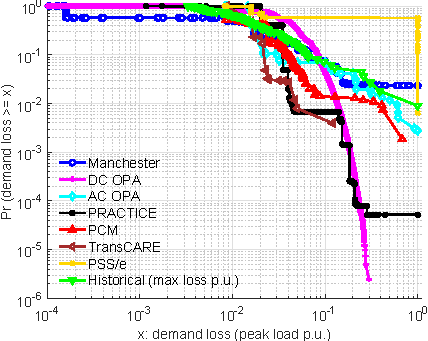
\includegraphics[width=0.6\linewidth]{Figs/QSS_ccdf.pdf}
    \caption{Comparison of the blackout size probabilities predicted by different QSS methodologies~\cite{Benchmarking2018}}
    \label{fig:QSS_ccdf}
\end{figure}

It is interesting to note that, outside the field of cascading outage analysis, there has also been some concerns regarding static grid models. For example, RTE (the French TSO) is developing a tool called DynaFlow for steady-state computations using simplified time-domain simulation. Steady-states are usually computed with a power flow algorithm. But, additional loops are needed to account for controls used in power systems (\eg on-load tap changers, phase-shifter transformers, etc.). The order of which those loops are applied has an impact on the final state that is computed. This order was previously defined using heuristics and experience, but this was becoming complex with the increasing number of loops, especially for large systems (and power systems becoming more ``smart''). DynaFlow showed more accurate results and ease of use~\cite{DynaFlow}. A similar tool called DynaWaltz was developed for long-term voltage stability~\cite{DynaWaltz}. % This tool replaced their previous QSS tool. DynaWaltz showed better accuracy than its predecessor while keeping similar computation times~\cite{DynaWaltz}.



\subsubsection{Methods with a dynamic grid model}
\label{sec:DynMethods}

Methods based on a dynamic grid model use time-domain simulations to assess the consequences of a given scenario. In this thesis, time-domain simulations are considered to be of the root-mean-square (RMS) type. Indeed, probabilistic security assessment methodologies based on RMS simulations are already strongly limited by computation time and thus cannot afford to use electromagnetic transient (EMT) simulations. The need for EMT simulations is driven by the increasing penetration of converter-interfaced generation (wind, solar), load (electric vehicle chargers), and transmission elements (HVDCs, STATCOMs, etc.) that have very fast dynamics (bandwidth from a dozen of Hz up to hundreds of kHz). Power electronics can cause oscillations at these high frequencies and impact system stability. Modelling these oscillations requires the use of EMT models. However, such oscillations are generally caused by interactions at the plant level or between plants in a small geographical region; and actions to avoid these oscillations can largely be taken at the local (plant) level~\cite{AvoidEMT}. % Also, grid-forming controls of power electronics can be used to limit the loss of system inertia caused by the decreasing share of synchronous generator~\cite{GridFormingAreTheyTheKey}.
It is thus expected that RMS simulations will remain adequate to simulate the propagation of \emph{system-wide} disturbances at the system level for most scenarios. Co-simulation could also be used to simulate the part of the grid near the initial considered disturbance with an EMT tool (better modelling the initiation of the cascade), and the remaining of the grid with an RMS tool (to simulate the cascade propagation), to avoid the computational and tractability issues of full-system EMT simulations. Screening indicators could be used to identify the scenarios where there is a need for EMT modelling~\cite{CIGRE_book_screening}.

The main advantage of time-domain simulations (apart from considering dynamic stability issues) is that they allow for a conceptually easier modelling than static cascading simulators. Actually, the only additional challenges of using time-domain simulations in a probabilistic security assessment compared to a deterministic one are that (i) the system is simulated further from normal operations, challenging the accuracy of the models, and (ii) protection systems (and their possible failures and misoperations) play a much more significant role and need to be modelled explicitly. Sensitivity studies are very important to control the first point, and chapter~\ref{ch:protections} is dedicated to the second.

The drawback of dynamic methods is significantly larger computation times and data requirements. Compared to static methods, the additional necessary data are mainly linked to (i) the dynamic models of generators, loads, etc. and (ii) the models of protections. Data for the first point is generally available to TSOs as stability studies are performed routinely, but the validity of existing models might be challenged when simulating the system during severe disturbances.  The second point requires data regarding the failure modes and failure rates of protection systems (that can be difficult to estimate) and the protection settings (that should be available but introduce additional data handling issues).

Moreover, using time-domain simulations does not resolve the fact that cascading outages can be very sensitive to modelling uncertainties and in particular to the timing of protection system operations. Multi-paths methods are still needed to handle this issue. Different techniques have been developed in the literature and are reviewed below.

In~\cite{SongThesis, SongPaper, Preece1000RandomDynN-2}, protections systems are modelled as perfectly reliable: they never fail and always trip at the expected threshold. This thus does not consider the sensitivity of cascading outages and does not allow for the consideration of N-k outages caused by protection failures. N-1-1 contingencies were considered instead (although referred to as N-2 contingencies).

The Pacific Northwest National Laboratory (PNNL) developed a tool called Dynamic Contingency Analysis Tool (DCAT) for security assessment of power systems~\cite{DCATphase1, DCATphase2}. In this tool, after the initiating contingency, the evolution of the system is computed using dynamic simulation. Protections are modelled explicitly in the simulation, and when one protection activates, the simulation is stopped and the state of the system is saved. From this save, two simulations are run, one where the protection actually operates, and one where it fails to (representing failure of a circuit breaker to open on demand). The limitation of this method is that only missing protection operations are considered. Unwanted operations are not considered. Also, the sensitivity of cascading outages is not considered. Moreover, the reports did not show any example of application using the ``protection misoperation'' functionality. There was also no discussion on the impact on the computational burden of this feature. But, in~\cite{DCAT_2023}, it is shown that it takes around one day with a 24-core computer to simulate 1465 scenarios (combination of an initial system state and contingency) on the WECC system (west US) using DCAT. The scenarios consisted in a combination of 2 contingencies with around 600 system states and in a combination of 213 contingencies with 1 system state. It was not possible to perform a systematic analysis with both many contingencies and many system states.

A particularity of DCAT is that is uses both dynamic and static simulations. Indeed, it uses dynamic simulations for the first 30 to 60 seconds after the initial contingency. If the system is deemed dynamically stable (\ie if no event occurs during the last dozen of seconds of the dynamic simulation), the tool then switches to (single-path) static simulation. When an event occurs in the static simulation (\eg a corrective action), the tools switches back to dynamic simulation. This allows for the simulation of the system over long time scales (minutes to hours to account for \eg line overloads) with reasonable computation time while still accurately simulating faster phenomena (\eg frequency stability in the 100ms-10s range). Another way to achieve this is via the use of time-domain simulators with a variable integration time-step such as Eurostag~\cite{STAG}.

Ref.~\cite{Haarla, GridPSA} proposed a methodology based on event trees. An example of event tree is shown in Figure~\ref{fig:eventTree}. An event tree starts at a given initiating event (a permanent line fault in the left of the figure). The event tree then branches when subsequent events (typically protections against the initial event) are possible. Upward branches are usually associated with the occurrence of an event (\eg protection operates successfully), and downward branches with the non-occurrence of the event (\eg protections fails to operate). The event tree thus generates a number of scenarios whose frequency and consequences can be estimated. The frequency of a branch is computed as the frequency of the initial event multiplied by the probability of the subsequent (non-)events. To complement event trees, fault trees can be used to model common-mode failures, they are presented in more details in dedicated literature~\cite{FaultTreeHandbook}. Consequences are estimated using dynamic simulations. The limitation of this method is that the event tree is built prior running the simulations. The analyst thus has to predict which protections will be activated. In practice, this is only possible for the protections that isolate the fault (\eg protections at both sides of the line and backups for these protections). This method only allows to consider some protection failure modes (although it is quite good at it). Also, in this case, the sensitivity of cascading outages was not considered.

\begin{figure}
    \centering
    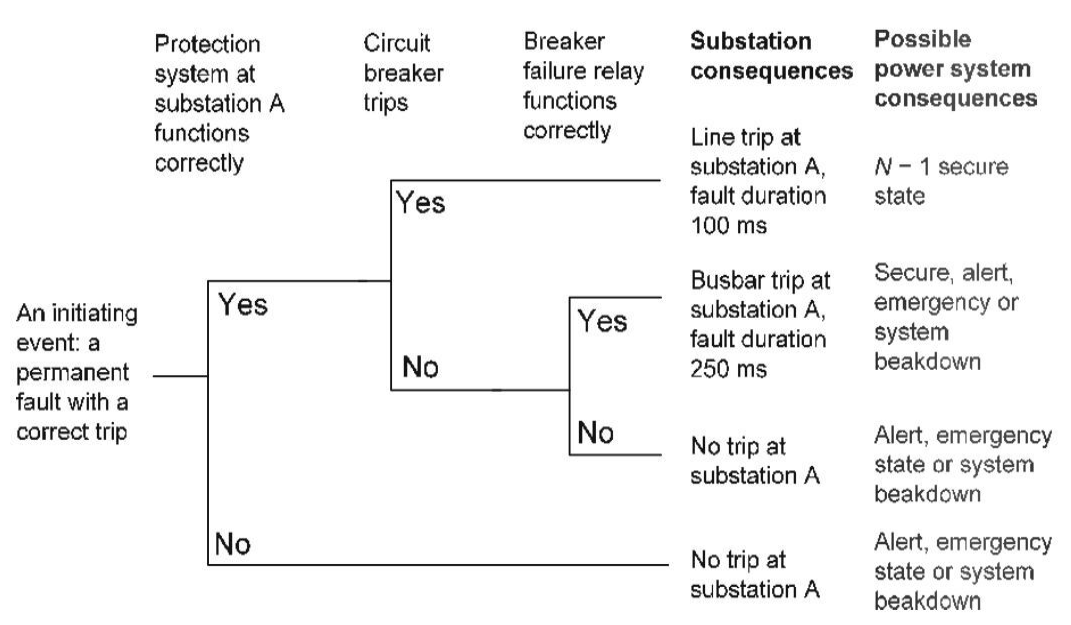
\includegraphics[width=0.8\linewidth]{Figs/EventTree.png}
    \caption{A simplified example of event tree for a line short-circuit~\cite{GridPSA}}
    \label{fig:eventTree}
\end{figure}

In~\cite{TwoLevelPSA, Faghihi}, an extension of event trees called dynamic event trees or continuous event trees have been used. In a dynamic event tree, branchings are not predefined by the analyst but naturally occur during the simulation following control actions. For example, similarly to DCAT, when one protection system operates, this can create two branches: one where the protection actually operates and one where it fails to. However, dynamic event trees are more general and can consider for example that, a protection system will trip when it observes a value slightly above or slight below the tripping threshold.

% In theory, a skilled analyst can alleviate the above limitations. He can use his expertise and/or simulation results to identify events that can occur during the system evolution. Also, if the order and/or timing of events is of importance, he can add additional events to consider them (\eg split ``event A occurs" in ``events A occurs before \(t=\)~5~s" and ``event A occurs after \(t=\)~5~s). It can however be difficult to compute the probabilities associated with those events. Also, the analyst should try to only consider the most critical scenarios to avoid an explosion of the size of the tree. So, in practice, this requires a lot of effort from the analyst. So-called dynamic event trees (DETs) have thus been developed with the objective to move most of the burden of proof of correctness from the analyst to the methodology. DETs are introduced in section~\ref{sec:dynamicReliability}.

% It should however first be noted while the above observations have mostly been made in the nuclear sector (wherefrom event trees originated)~\cite{LabeauTowards}, they are even more relevant for power systems. There is two main reasons for this. First, there are significantly more initiating events to consider. Indeed, one should consider at least hundreds of possible (\eg line) faults or even more depending on the size of the considered system (and the voltage level(s) considered). Also, for a given fault, multiple event trees should be built as the evolution of the system depends on the initial operating conditions. Second, a large number of events can occur after a disturbance, especially during fast cascading outages. Predicting those events as well as determining the importance of the timing and order of events might prove particularly complex.

This can be done by associating a probability density function to the threshold at which the protection will actually trip. Then, in theory, the dynamic event tree will create an infinity of branches to account for all the possible values at which the protection could trip. Of course, in practice, numerical schemes approximate this with a finite number of branches. Ref.~\cite{TwoLevelPSA, Faghihi, PierreMCDETprelim} proposed different numerical schemes and applied them to the analysis of cascading outages.

% Ref.~\cite{TwoLevelPSA} proposed two numerical schemes. The first is skeleton-based MC. In this methodology, the first step is to build a so-called skeleton. This is done in a similar way as in DCAT, \ie the evolution of the system is simulated, and when a protection is triggered, the simulation branches. In one branch, the protection actually operates, and in the second it fails to. Upon this skeleton, additional branches are grafted at discrete time steps before and after the original branchings points. These additional branches take into account measurement and setting errors of the relays. The probability of each of these additional branches depends on the evolution of system variables in the skeleton. For example, if the variable monitored by the protection ``hugs" the triggering threshold, the protection will be likely to trigger in a large time interval around its triggering time in the skeleton. On the other end, if the variable quickly goes beyond the threshold, the interval will be narrower. This methodology has been applied in~\cite{Faghihi}. The second method is MCDET. MCDET is a concatenation of MC and DDET (discrete DET, that can here be read as a synonym of skeleton). It was originally proposed in the nuclear domain by~\cite{MCDET}. In MCDET, continuous uncertainties (\eg measurement errors) are handled by MC. Then, for each MC sample, a skeleton is built. This skeleton handles the discrete uncertainties (\eg protection fails to operate). This method was however not fully implemented, and only preliminary results were presented~\cite{PierreMCDETprelim}.

% \TODO{Define correctly MCDET (no skeleton), see PEL comments}

Dynamic event trees are a very powerful modelling tool and can in principle account for any kind of uncertainty (sensitivity of cascading outages, missing trips, unwanted trips). However, solving them tend to be very computationally expensive, and their application in~\cite{TwoLevelPSA, Faghihi, PierreMCDETprelim} thus had to be limited to small-scale test systems.

% require more interactions with the simulator. They are thus used with custom simulators or simulators with powerful APIs.

It can be noted that, like DCAT, Ref.~\cite{TwoLevelPSA} uses both dynamic and static simulations but with a different approach. The approach is based on the observation that many cascades develop in two phases: a slow phase driven by thermal phenomena (overloads) and a fast phase driven by electrical phenomena (loss of stability). During the slow phase, the cascade is modelled using a static simulator. And when a possible instability is detected (possibly at the very start of the cascade if it directly does not go through a slow phase), dynamic event trees (with a time-domain simulator) are used to simulate the rest of the cascade. As time-domain simulation is more expensive than static simulation, scenarios simulated with the static method are first aggregated before being fed to the dynamic simulator. This allowed the authors to apply the methodology on a 73-bus system, but computation time limits the scalability.

The work of~\cite{EurostagHPC}, while not really a probabilistic security assessment, is interesting because it was applied to a large grid (the French power system). In this work, a brute-force approach was used and time-domain simulations were performed for around 7000 system states and 2000 N-1 contingencies (for a total of 14 million dynamic simulations). Authors did not study cascading outages, so protection systems (and their possible misoperations) were not modelled and the consequences of each scenario were labelled as either acceptable or unacceptable. The analysis took one day of computation time in a large high-performance computing (HPC) centre where 10,000 cores were reserved for the analysis. The computational burden would have been even higher if N-k contingencies were considered, highlighting the need to simulate as few scenarios as possible (while keeping acceptable accuracy).

% \cite{QimingChenThesis} % Not fully clear what he does

% \cite{MultiTimescaleMarkovianTree-ActuallyOnlyQSS}

\subsubsection{Other methods}
\label{sec:OtherMethods}

As discussed above, simulating cascading outages is complex and requires to make some modelling assumption. This has led some researchers to develop methods based on historical data. Indeed, historical data are by definition not dependent on modelling assumptions. From historical data, one can observe which elements played critical roles in past cascades. Those elements are good candidates for upgrades or replacements. However, historical data alone do not allow for the simulation of ``what if'' scenarios. For example, the benefits of a given upgrade cannot be estimated. This has led to the development of influence graphs models~\cite{CascadingInfluenceGraph} that are tuned to match historical data. The most famous model of this category is the Oak Ridge-PSERC-Alaska (OPA) model~\cite{OPA2019}. The issue when building models from historical data are that these data consist mainly in small cascades as large blackouts are (hopefully) rare. However, large blackout, while rare, contribute to a large share of the total risk~\cite{CascadingMethodoAndChallenges} and are more likely to lead to fast cascades that are poorly represented in historical data~\cite{cascadeAcceleration}. Also, the accuracy of these models have been questioned~\cite{TopologicalModelsBad}. And finally, relying too much on (rare) historical data might prove dangerous knowing that power systems are currently facing large changes to facilitate the energy transition.

Another kind of methods used in the context of probabilistic dynamic security assessment is the use of machine learning techniques as reviewed in~\cite{MLEfthymios}. However, for now, these tools are only able to predict if a given scenario will be stable or not (and possibly margins to stability). They cannot provide with an estimation of the consequences nor predict how a cascade could propagate. They are thus mostly proposed to be used in real-time operations (after being trained offline) as they are fast (once trained) and give simple predictions (system is stable or not). In a planning horizon, they are less useful due to their high training time, and because they cannot quantify the consequences of scenarios and thus cannot evaluate the risk.


\subsection{Evaluating the monetary cost of blackouts}
\label{sec:blackout_cost}

When a given scenario is simulated, the simulation will give an estimate of its consequences in terms of MW of load that is deenergised at the end of the cascade. However, it would be useful to also have an estimation of what would be the societal cost of such scenario as it would allow TSOs to more easily compare the impact of any risk-mitigation action (change of operating rule, construction of new line, etc.) to the cost of its implementation.

This is usually done in two steps. The first step is to translate the amount of MW of deenergised load into the energy not supplied (ENS) in MWh. This requires some reenergising model, \ie to estimate how long it takes to reenergise the full grid after a cascade. And the second step is to translate this ENS into a monetary cost. The reenergising time depends on the reenergising strategy used which vary greatly among TSOs as this task involves safety concerns (once a network element is in an outage state, the TSO has to make sure that reenergising it does not endanger anything or anyone)~\cite{ENTSOE-PSA_second_report}. Thus, in this thesis, a simple model from~\cite{TwoLevelPSA} is used.

This model is based on historical blackouts and on the observation that the time to full recovery after a blackout is loosely proportional to the percentage of the total load that is deenergised as shown in Figure~\ref{fig:restoration_time}. This means that it takes more time to recover from larger blackouts which partly explains why large blackouts, although rare, can significantly contribute to the total risk of load shedding~\cite{CascadingMethodoAndChallenges}. It is also possible to account for the fact that the reenergising process if fast at the start as the main load centres are reconnected and slow at the end when only remote customers remain to be connected. In~\cite{TwoLevelPSA}, this is done using an exponential recovery model.

\begin{figure}
    \centering
    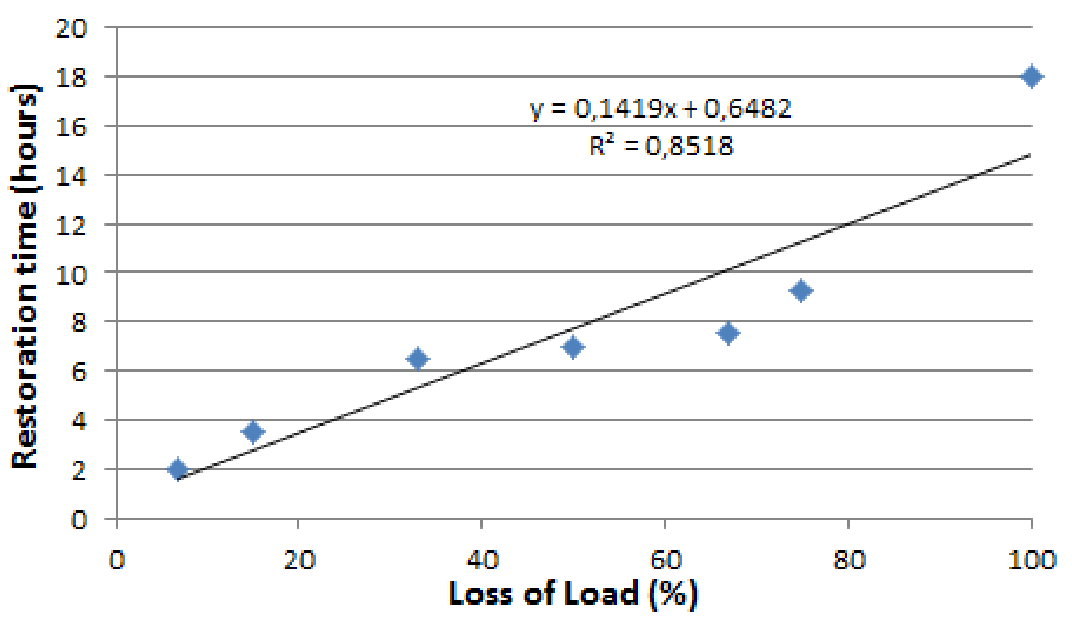
\includegraphics[width=0.6\linewidth]{Figs/RestorationTime.png}
    \caption{Restoration time of historical blackouts depending on their size~\cite{TwoLevelPSA}}
    \label{fig:restoration_time}
\end{figure}

The value of lost load is defined as the monetary value that an average consumer places on a kWh of energy not served without notice. Table~\ref{tab:VOLL} shows how this value depends on the duration of the interruption~\cite{VOLL}. It should be noted that the cost of energy not served is much larger than the cost of energy. Indeed, Table~\ref{tab:VOLL} gives values of the order of 20,000€/MWh while the price of electricity on the bulk energy market is of the order of 50€/MWh. Another simple way of estimating the value of lost load that is to consider that a one-day blackout of a country costs a 365th of its gross domestic product.

\begin{table}
    \centering
    \caption{Value of lost load, adapted from~\cite{VOLL}}
    \label{tab:VOLL}
    \begin{tabular}{@{}ll@{}}
    \toprule
    Interruption duration & Value of the loss of load \\ \midrule
    1 min  & 571 €/kWh \\
    20 min & 61 €/kWh \\
    1h     & 39 €/kWh \\
    4h     & 30 €/kWh \\
    8h     & 27 €/kWh \\
    24h    & 13 €/kWh \\ \bottomrule
    \end{tabular}
\end{table}

Based on the above reenergising model and value of lost load, the following relation can be derived between the percentage of load disconnected after a cascade and the cost for society.

\begin{equation}
    \label{eq:VOLL}
    C = \frac{3}{H} \int_0^H t \; e^{\frac{-3t}{H}} LOL \; VoLL(t) \; dt
\end{equation}
\noindent where \(H\) is the total restoration time of the blackout (estimated from Figure~\ref{fig:restoration_time}), \(LOL\) is the percentage of deenergised load at the start of the restoration process (thus \(e^{\frac{-3t}{H}} LOL\) is the percentage of deenergised load \(t\) hours after the start of the restoration), and \(VoLL\) is the value of lost load (from Table~\ref{tab:VOLL}).


\section{Conclusion}
\label{sec:security-conclusions}

This chapter has introduced the concept of power system security and the causes that can lead to a lack of security. It then presented the currently-used \emph{deterministic} methods for power system security assessment, discussed their limitations and justified the need for \emph{probabilistic} methods. Probabilistic approaches are more powerful than deterministic ones, but this comes at the cost of added complexity. In particular,

\begin{itemize}
    \item Probabilistic methods consider high-order contingencies that are neglected in deterministic assessments. They thus require to model the causes of these high-order contingencies and to estimate their frequency of occurrence.
    \item Probabilistic methods perform the security assessment on a large set of possible system states instead of on a few representative ones. This requires to generate many likely system states and to estimate their respective probability while accounting for spatio-temporal correlations between renewable energy availability at different point in the network, load, etc.
    \item Probabilistic methods quantify the potential consequences of contingencies in terms of energy not served or costs for society while deterministic methods limit the analysis to a dichotomous approach (the contingency is secure or not). They thus put higher priority on contingencies that lead to complete blackouts compared to the ones that simply lead to minor consequences. However, quantifying the consequences of a contingency requires simulating the propagation of large cascading outages which is very challenging.
\end{itemize}

As discussed in section~\ref{sec:contingencies}, a large share of high-order contingencies (and resulting historical blackouts) are caused by (hidden) failures of protection systems. The modelling of protection systems and their failure modes is thus tackled in chapter~\ref{ch:protections}.

The second challenge tackled in this thesis is the simulation of cascading outages. As discussed in section~\ref{sec:cascading}, two main types of methods have been developed for the simulation of cascading outages: quasi-steady-state simulation and time-domain simulation. However, there is still no consensus on how to model ``race conditions'' between different cascading mechanisms in static simulations, and their relevance is decreasing as a growing share of cascading outages are purely driven by fast stability phenomena that can only be adequately modelled using time-domain simulations~\cite{cascadeAcceleration}.

Even when using time-domain simulations, simulating cascading outages stays a challenge as (i) it requires to simulate the system in very degraded conditions, and (ii) the evolution of a cascade might be very sensitive to modelling uncertainties because small changes in the timing of protection system operations can vastly change the cascading path. Protection systems are typically not modelled in deterministic security assessments because they only operate in degraded states. However, they are a key driver in the evolution of cascading outages and are thus discussed in chapter~\ref{ch:protections}. The high sensitivity of cascading outages to protection system behaviour is also discussed in that chapter. % Chapter~\ref{ch:SPS} then focuses on system integrity protection schemes, a particular kind of protection system that can be used to increase system security.

Another important driver of cascading outages that is usually not very well modelled in deterministic assessment is the behaviour of distribution systems. Indeed, with the increasing share of distributed energy sources (rooftop solar, small- and medium-sized wind farms), distribution systems are playing a more and more active role in the stability of power systems. However, distributed energy sources, especially legacy installations with limited fault ride-through capabilities, tend to disconnect themselves during system disturbances, further weakening the system at the worst possible time. The modelling of distribution systems and their impact on transmission system stability is thus discussed in chapter~\ref{ch:distrib}.

Finally, because probabilistic methods consider many scenarios (combinations of possible initial system states and contingencies), and because time-domain simulations of individual scenarios are computationally expensive, it is necessary to limit as much as possible the number of simulated scenarios to be able to perform the analysis with reasonable computational resources. But of course, this should not jeopardise accuracy. Chapter~\ref{ch:DPSA} propose some methods to tackle this issue. Also, it discusses what can be done with the results a probabilistic security assessment.
